\section{Evaluation}

\subsection{Experimental Setup}
\label{sec:setup}
% Describe the overall experimental setup, including the hardware used, the models / applications and the datasets.


% \begin{figure*}
% 	\centering
% 	\begin{subfigure}[b]{0.45\textwidth}
% 		\centering
% 		\includegraphics[width=\textwidth]{chapters/roomie/tmp/JetsonNano/clean_workdir_avg_response_time/alexnet-convnext-densenet-efficientnet-googlenet-inception-mobilenet-mobilenet-resnet-resnet-resnet-shufflenet-squeezenet-wide/goodput.png}
% 		\caption{\textbf{Jetson Xavier} 12$\times$ classificaton models}
% 		\label{fig:isolation}
% 	\end{subfigure}
% 	\hfill
% 	\begin{subfigure}[b]{0.45\textwidth}
% 		\centering
% 		\includegraphics[width=\textwidth]{chapters/roomie/tmp/JetsonNano/clean_workdir_avg_response_time/alexnet-convnext-densenet-googlenet-inception-mobilenet-mobilenet-resnet-shufflenet-squeezenet/goodput.png}
% 		\caption{\textbf{Jetson Xavier} 10$\times$ classification models}
% 		\label{fig:colocation}
% 	\end{subfigure}
% 	\label{fig:three graphs}
% \end{figure*}



\paragraph{Baselines.} We evaluate \roomie{} against two different state-of-the-art baselines: INFaaS and Usher. INFaaS performs accuracy scaling by scaling variants within the same worker to meet demand. Usher, on the other hand, groups compute-heavy models with memory-heavy models within a group. We have used different models from two family groups, namely classification and detection, to evaluate our solution and baselines. We consider that each incoming query is intended for a single inference model.

\paragraph{Deployment Infrastructure.} We conducted our experiments using two distinct deployment types: a cluster of Jetson Nanos and a cluster of larger GPUs. The first consisted of $3\times$ machines equipped with $4\times$ Nvidia \textit{A100-SXM4-40GB (40 GiB)}. The second consisted of $12\times$ Nvidia Jetson AGX Xavier GPUs. Each GPU is assigned to a docker to form a server, making a total of 12 servers for each deployment. We also used $2\times$ HPE Proliant DL360 Gen10+ the client requesting the model and a controller responsible for serving requests to workers. The full specifications are presented in \Cref{tab:serve_config}.

\begin{table}
	\centering
	\begin{tabular}{p{2cm}p{3cm}p{3cm}}
		\toprule
		\textbf{Model}            & \textbf{CPU}                                & \textbf{GPU}                                                 \\
		\toprule

		Nvidia Jetson AGX Xavier  & 1 CPU/node, 8 cores/CPU                     & Nvidia AGX Xavier, CC~\footnote{CC: Compute capability}: 7.2 \\

		\midrule

		HPE Proliant DL360 Gen10+ & x86\_64, 2.40GHz, 2 CPUs/node, 16 cores/CPU &                                                              \\

		\midrule

		Apollo 6500 Gen10+        & x86\_64, 1 CPU/node, 32 cores/CPU           & $4\times$ Nvidia A100-SXM4-40GB (40 GiB), CC: 8.0            \\

		\midrule

		DL360 Gen10+              & x86\_64, 2.60GHz, 2 CPUs/node, 32 cores/CPU &                                                              \\

		\bottomrule
	\end{tabular}
	\caption{Server configuration used for experiments.}
	\label{tab:serve_config}
\end{table}

\paragraph{Datasets.} We evaluated our system and baseline methods using both synthetic and real-world workloads. For the real workload, we adopt the Twitter trace 2020 dataset~\cite{twitterStreamTrace2020}, as it is particularly suitable for modeling inference services, as tweets are commonly subjected to deep neural network (DNN) processing before publication~\cite{francisco2021infaas,ahmad2024proteus}. Since the trace is aggregated at a coarse temporal granularity of one second, we apply a Poisson process to model intra-second arrival times and use a Zipf distribution to distribute queries among models, in line with established methodology~\cite{francisco2021infaas,ahmad2024proteus}.
For synthetic workloads, we generated average request rates per second using a Gaussian process and applied the same Zipf-based model allocation. To ensure our evaluation captures a broad spectrum of inference behavior, we selected a diverse and representative set of deep neural network (DNN) models. These include both high-performance classification architectures and widely adopted object detection frameworks, enabling us to rigorously assess system behavior under varied computational and latency profiles. The full list of models is summarized in~\Cref{tab:dnn-models}, reflecting the breadth and relevance of our evaluation design.

\begin{table}[h]
	\centering \caption{Categorization of Deep Neural Network Models Used in Evaluation} \label{tab:dnn-models}
	\begin{tabular}{p{4cm}p{6cm}}
		\hline
		\textbf{Category} & \textbf{Models}
		\\ \hline
		Classification Models &
		\texttt{vgg19},
		\texttt{alexnet},
		\texttt{maxvit\_t},
		\texttt{resnet152},
		\texttt{googlenet},
		\texttt{densenet201},
		\texttt{squeezenet1\_1},
		\texttt{mobilenet\_v3\_large},
		\texttt{shufflenet\_v2\_x2\_0},
		\texttt{inception\_v3},
		\texttt{wide\_resnet101\_2},
		\texttt{resnext101\_32x8d},
		\texttt{efficientnet\_v2\_l},
		\texttt{convnext\_large}
		\\ \hline
		Object Detection Models &
		\texttt{ssd300\_vgg16},
		\texttt{fcos\_resnet50\_fpn},
		\texttt{retinanet\_resnet50\_fpn\_v2},
		\texttt{fasterrcnn\_resnet50\_fpn\_v2},
		\texttt{ssdlite320\_mobilenet\_v3\_large}
		\\ \hline 
	\end{tabular}
\end{table}

% We evaluated our system and baselines using synthetic and real workloads. For the real workload, we used Twitter's public traces from 2020~\cite{twitterStreamTrace2020} as was done in the state-of-the-arts. The trace is representative of the workloads that an inference service system would expect to see, since tweets are likely to be run through an inference model before being published~\cite{francisco2021infaas,ahmad2024proteus}. Since these traces are collected and aggregated at the granularity of seconds, we use a Poisson process to determine query arrival times within each second and use the Zipf distribution to allocate queries between models as in previous work~\cite{ahmad2024proteus,francisco2021infaas}. For synthetic data, we use a Gaussian process to determine the average number of requests per second, which we distribute in the same way as for the real workload.


% We evaluated our system and baselines using synthetic and real workloads. For the real workload, we used Twitter's public traces from 2020~\cite{twitterStreamTrace2020} as was done in the state-of-the-arts. The trace is representative of the workloads that an inference service system would expect to see, since tweets are likely to be run through an inference model before being published~\cite{francisco2021infaas,ahmad2024proteus}. Since these traces are collected and aggregated at the granularity of seconds, we use a Poisson process to determine query arrival times within each second and use the Zipf distribution to allocate queries between models as in previous work~\cite{ahmad2024proteus,francisco2021infaas}. For synthetic data, we use a Gaussian process to determine the average number of requests per second, which we distribute in the same way as for the real workload. About the models we used for our evaluations are: alexnet, squeezenet1_1, mobilenet_v3_large, shufflenet_v2_x2_0, googlenet, vgg19, inception_v3, wide_resnet101_2, resnext101_32x8d, resnet152, maxvit_t, densenet201, efficientnet_v2_l, convnext_large, fcos_resnet50_fpn, retinanet_resnet50_fpn_v2, fasterrcnn_resnet50_fpn_v2, ssd300_vgg16, ssdlite320_mobilenet_v3_large.


\paragraph{Evaluation Metrics.} To evaluate the effectiveness of each DNN deployment strategy, the assessment focused on four key performance indicators. Response time measured how quickly the models delivered results, which is a critical indicator of real-time performance. The processing rate indicated the percentage of requests successfully processed, highlighting the reliability of the system for different workloads. Throughput measured the number of requests processed in a given time frame, providing insight into overall capacity and scalability. Finally, GPU utilization monitored the degree of hardware resource usage during model execution.


\subsection{Performance Evaluation of Cloud-Based GPU Cluster Solutions}

To assess the effectiveness of our proposed deployment strategy, we conducted a comprehensive evaluation using a cloud-based GPU cluster comprising 12$\times$ GPUs and all deep neural network (DNN) models detailed in~\Cref{tab:dnn-models}. The experiments were performed using two distinct datasets: real-world Twitter data and synthetically generated data. These synthetic workloads were constructed to mimic real-world traffic patterns while allowing precise manipulation of query rates. This enabled a more granular analysis of system behavior under stress. These datasets were used to simulate varying workload intensities, beginning with low traffic levels that all models could handle and gradually increasing until system saturation was observed.

\paragraph{Evaluation on Twitter dataset.}

\begin{figure*}
	\begin{minipage}[t]{.24\linewidth}
		\centering
		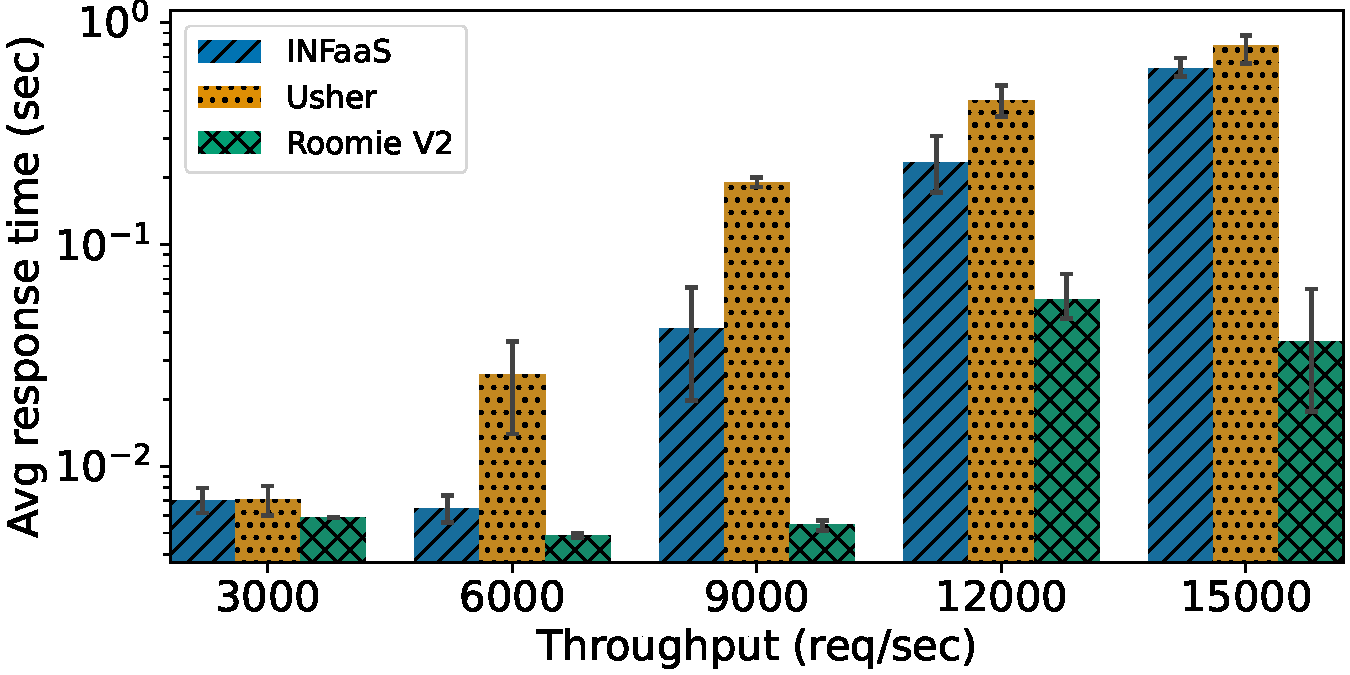
\includegraphics[width=\linewidth]{chapters/roomie/images/NvidiaA100/twitter-all-models/response_time.pdf}
		\subcaption{Response time.}
	\end{minipage}
	\hfill
	\begin{minipage}[t]{.24\linewidth}
		\centering
		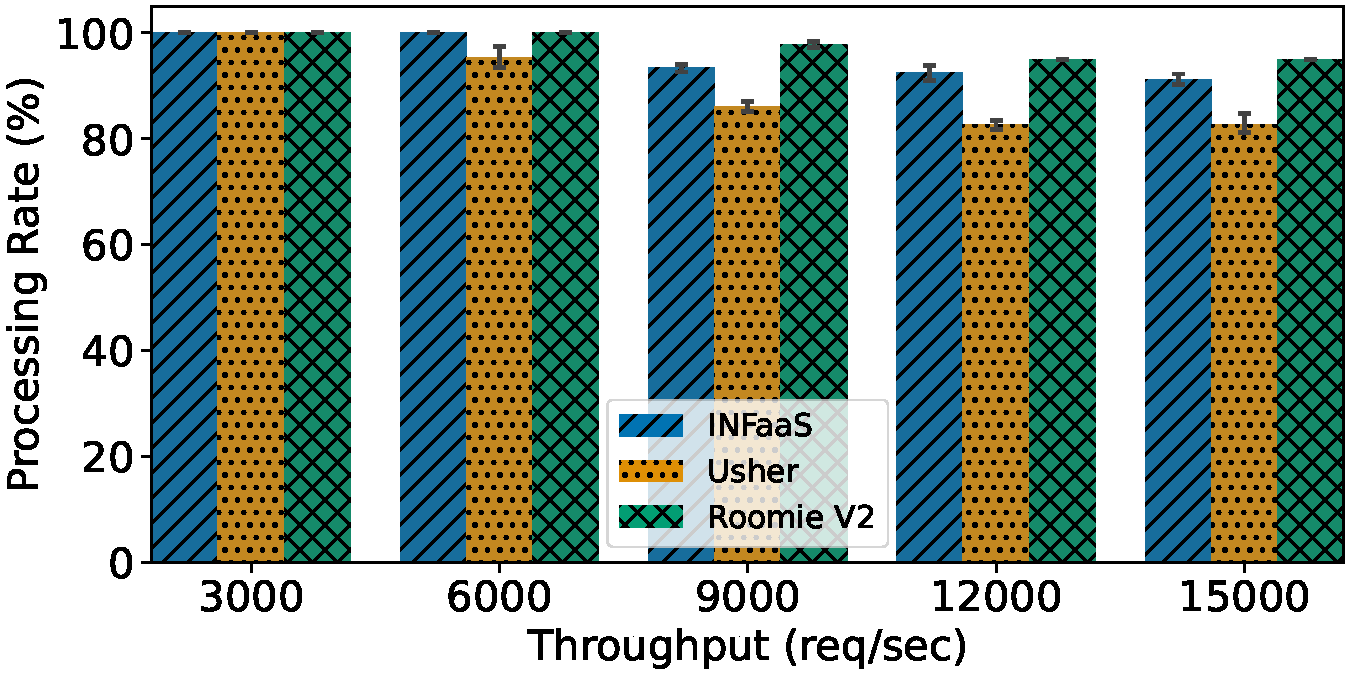
\includegraphics[width=\linewidth]{chapters/roomie/images/NvidiaA100/twitter-all-models/normalized.pdf}
		\subcaption{Processing rate.}
	\end{minipage}
	\hfill
	\begin{minipage}[t]{.24\linewidth}
		\centering
		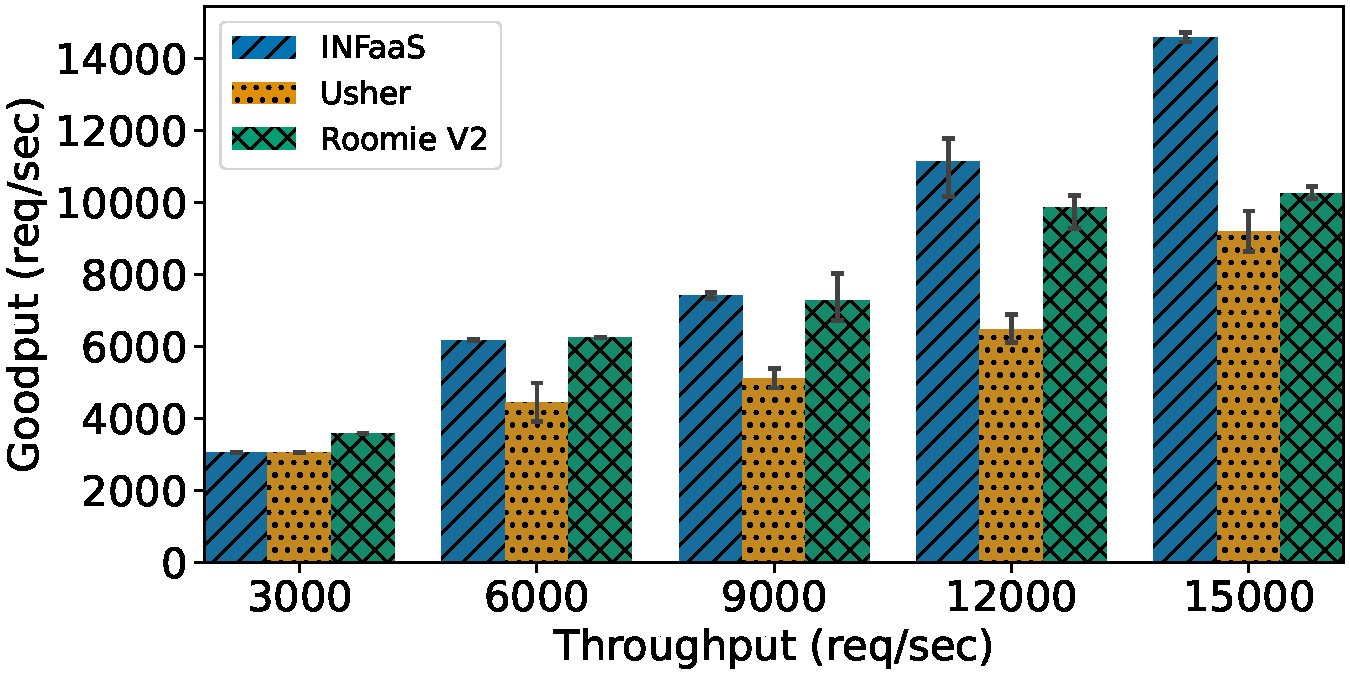
\includegraphics[width=\linewidth]{chapters/roomie/images/NvidiaA100/twitter-all-models/goodput.pdf}
		\subcaption{Goodput.}
	\end{minipage}
	\hfill
	\begin{minipage}[t]{.24\linewidth}
		\centering
		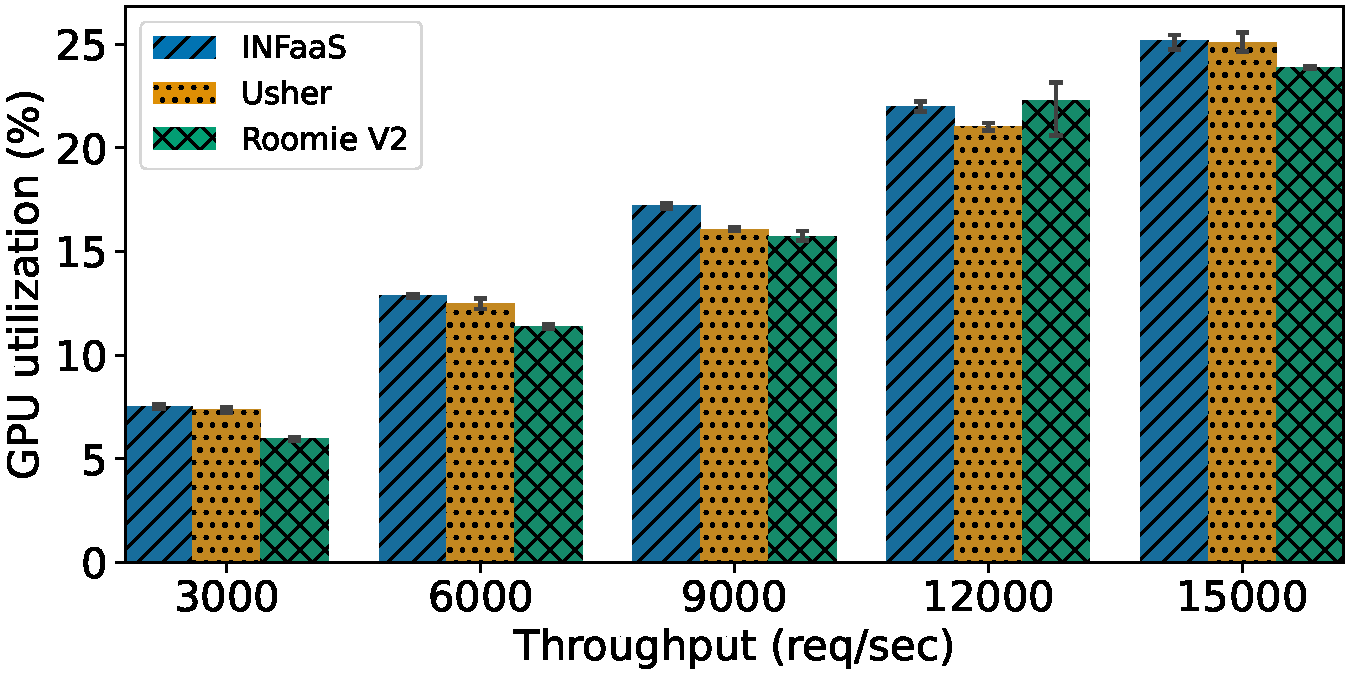
\includegraphics[width=\linewidth]{chapters/roomie/images/NvidiaA100/twitter-all-models/gpu_utilization.pdf}
		\subcaption{GPU utilization.}
	\end{minipage}
	\caption{\roomie achieves up to 17$\times$ faster response times while delivering similar processing rates in a cloud-based evaluation using the Twitter dataset, outperforming INFaaS and Usher under high workload conditions.}
	\label{fig:NvidiaA100/twitter-all-models}
	\vspace{-3mm}
\end{figure*}

\Cref{fig:NvidiaA100/twitter-all-models} shows the performance results obtained from the Twitter database. Under low workload conditions, all approaches showed comparable response times. However, as the workload increased, significant performance disparities emerged. Notably, Roomie achieved response times up to 17× faster than rival solutions and maintained a processing rate above 97\%. In contrast, Usher's strategy of co-locating large models with lightweight models failed to deliver satisfactory performance under high load, resulting in increased latency and reduced goodput. INFaaS, which scales DNNs on workers already hosting a copy, showed moderate goodput performance. However, this approach is agnostic to model interference, leading to latency increases of up to 17× and a decline in processing rate.

Interestingly, despite low GPU utilization across all approaches, we observe a significant increase in response time as workload intensifies. This counterintuitive behavior can be attributed to the saturation of large models, which become unable to keep pace with incoming queries. As these models reach their computational limits, they begin to queue requests, leading to latency explosions—even though the GPU itself remains underutilized. Additionally, interference between co-located models can further degrade responsiveness, compounding delays without a corresponding rise in GPU activity. One potential mitigation strategy is to increase batch sizes, which can improve utilization by amortizing overhead across multiple queries. However, this approach introduces a trade-off: larger batches may inflate response times, making it unsuitable for latency-sensitive applications. These findings underscore the need for deployment strategies that go beyond raw utilization metrics and account for model saturation dynamics and cross-model interference.


\paragraph{Evaluation on synthetic dataset.}

\begin{figure*}
	\begin{minipage}[t]{.24\linewidth}
		\centering
		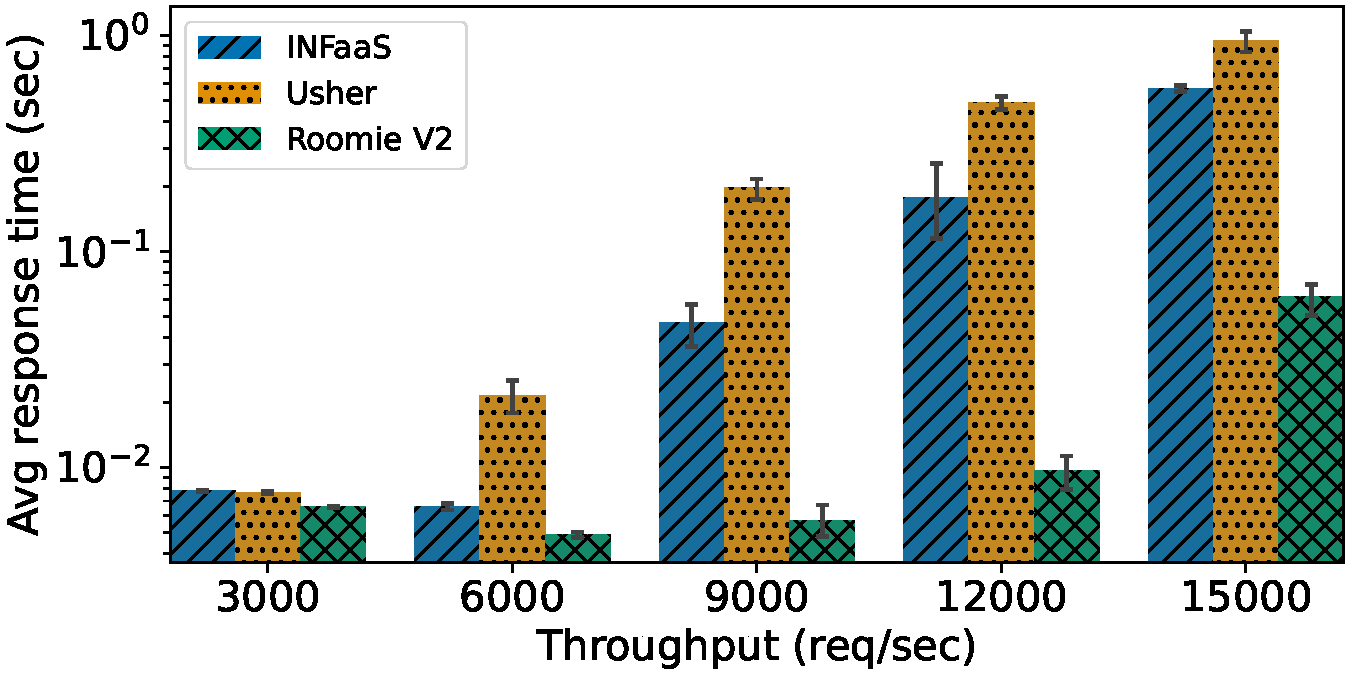
\includegraphics[width=\linewidth]{chapters/roomie/images/NvidiaA100/synthetic-all-models/response_time.pdf}
		\subcaption{Response time.}
		\label{fig:NvidiaA100/synthetic-all-models/response-time}
	\end{minipage}
	\hfill
	\begin{minipage}[t]{.24\linewidth}
		\centering
		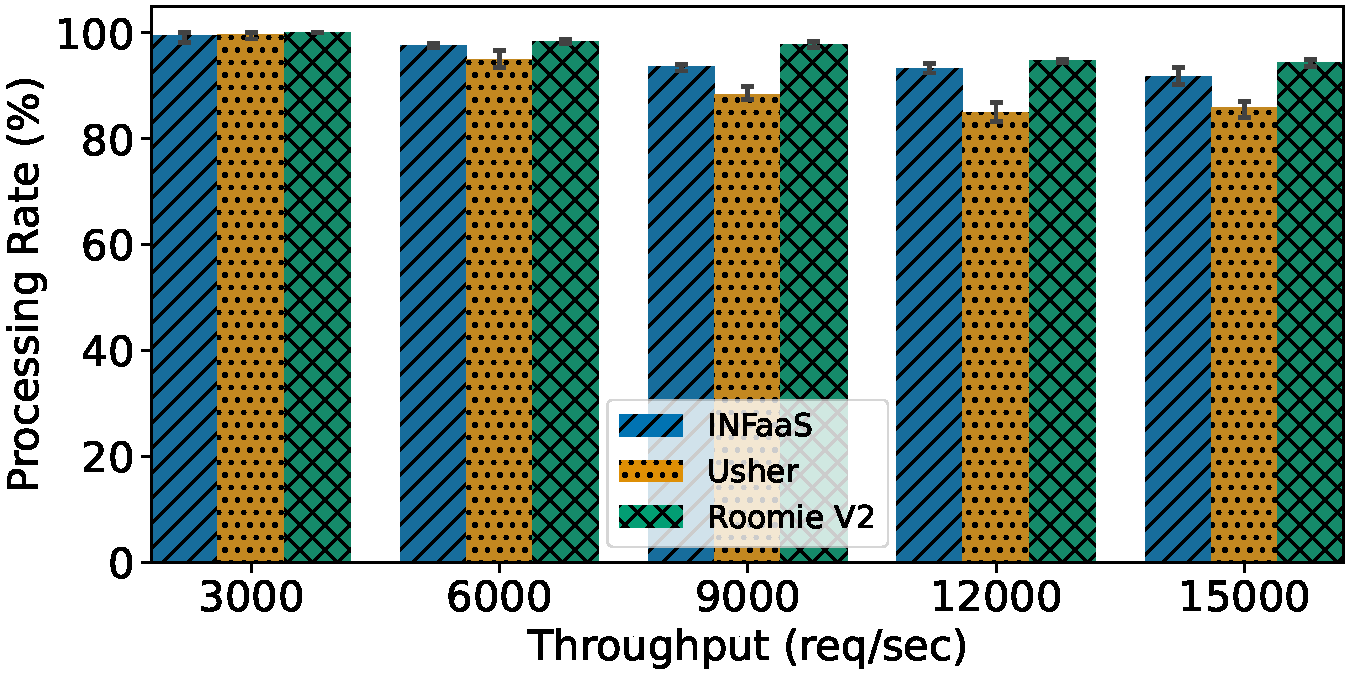
\includegraphics[width=\linewidth]{chapters/roomie/images/NvidiaA100/synthetic-all-models/normalized.pdf}
		\subcaption{Processing rate.}
	\end{minipage}
	\hfill
	\begin{minipage}[t]{.24\linewidth}
		\centering
		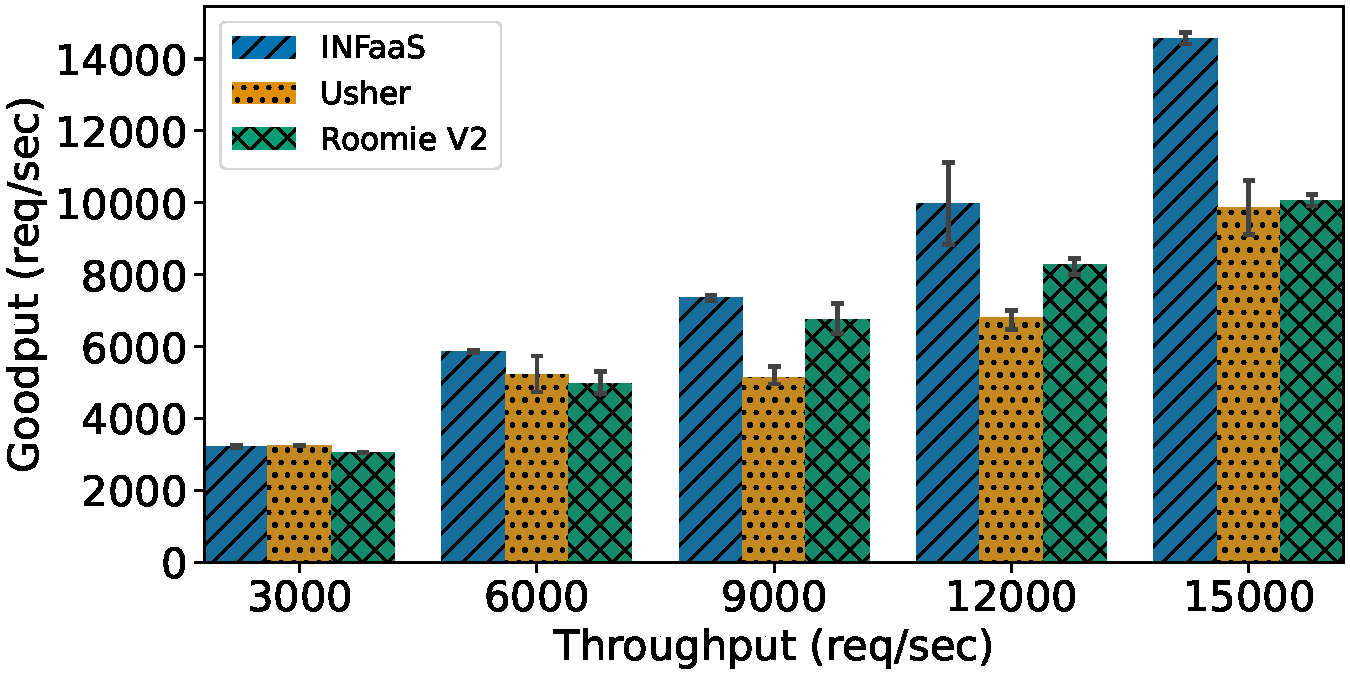
\includegraphics[width=\linewidth]{chapters/roomie/images/NvidiaA100/synthetic-all-models/goodput.pdf}
		\subcaption{Goodput.}
	\end{minipage}
	\hfill
	\begin{minipage}[t]{.24\linewidth}
		\centering
		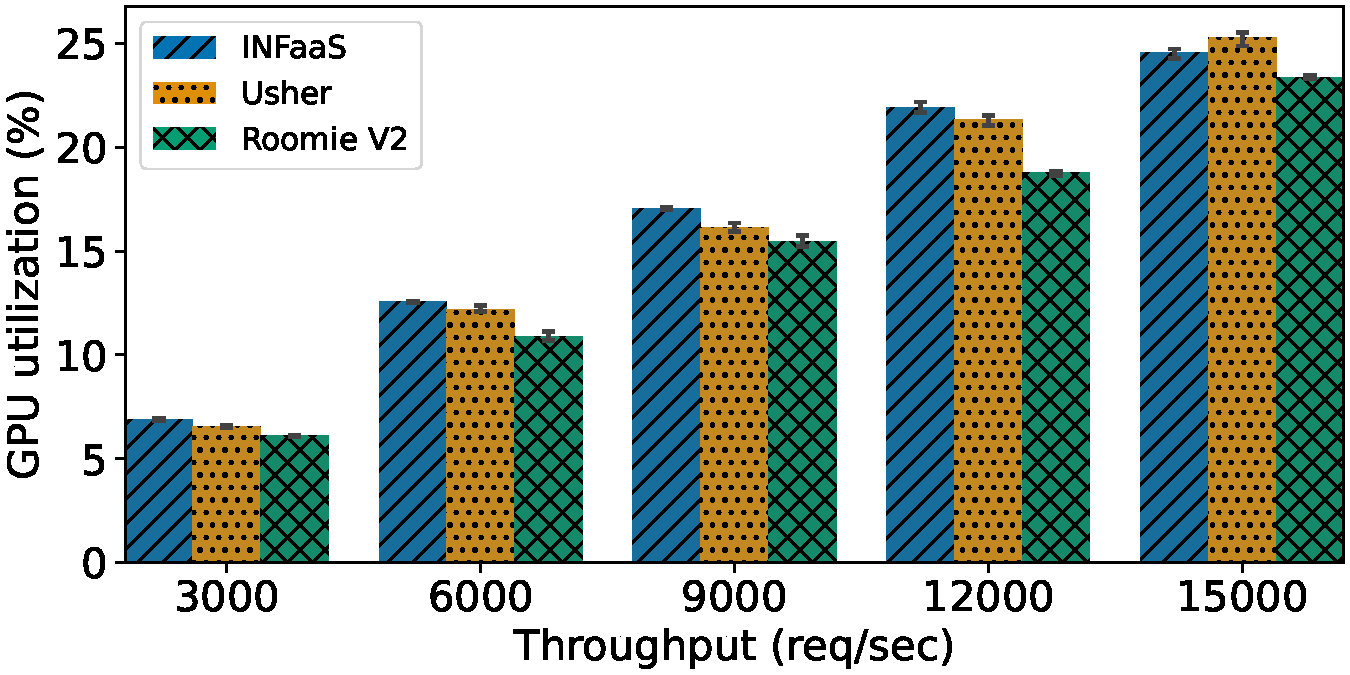
\includegraphics[width=\linewidth]{chapters/roomie/images/NvidiaA100/synthetic-all-models/gpu_utilization.pdf}
		\subcaption{GPU utilization.}
	\end{minipage}
	\caption{In cloud-based evaluation using synthetic workloads, Roomie yields 9.2× faster response time and higher processing rate, confirming its deployment efficiency in controlled stress scenarios.}
	\label{fig:NvidiaA100/synthetic-all-models}
	\vspace{-3mm}
\end{figure*}


\Cref{fig:NvidiaA100/synthetic-all-models/response-time} illustrates the results of the evaluation conducted with a synthetic dataset designed to emulate diverse and controlled workload scenarios.\\
The performance trends observed with the synthetic dataset closely mirrored those seen with the Twitter data. Roomie consistently outperformed other deployment strategies, achieving a 9.2× reduction in response time and superior throughput and processing rates. These gains are attributed to Roomie's intelligent model deployment and colocation strategy, which minimizes interference and maximizes resource efficiency.

Overall, across both datasets, Roomie demonstrated robust performance under varying workload conditions. It consistently achieved lower response times—up to 17× faster—and higher throughput than competing approaches, validating its effectiveness in cloud-based GPU environments.



\subsection{Performance Evaluation on Edge Devices Using Jetson Xavier GPUs}

To further validate our approach, we conducted a second set of experiments using a cluster of 12 Jetson Xavier GPUs, representative of resource-constrained edge computing environments. As in the cloud-based evaluation, we deployed 12 models (from~\Cref{tab:dnn-models}) and tested performance using Twitter data and synthetic data, gradually increasing the workload intensity.

\paragraph{Evaluation on twitter dataset.}

\begin{figure*}
	\begin{minipage}[t]{.24\linewidth}
		\centering
		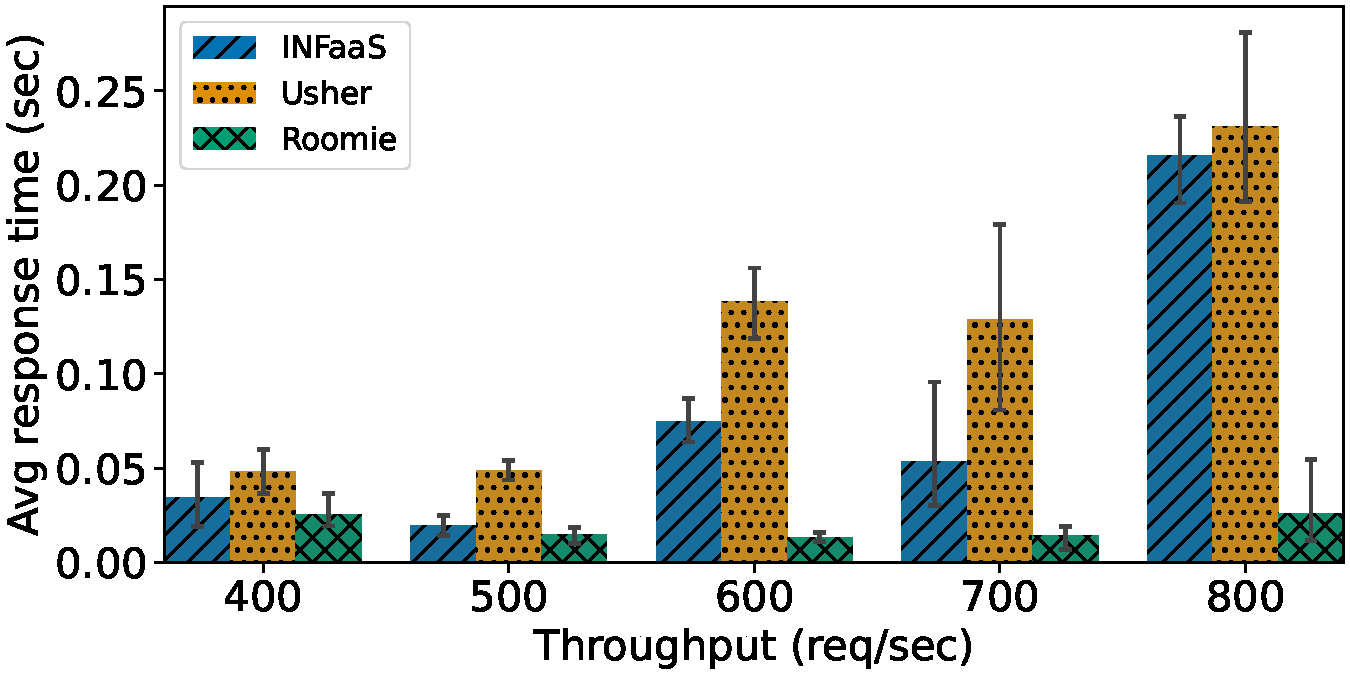
\includegraphics[width=\linewidth]{chapters/roomie/images/JetsonNano/twitter-all-models/response_time.pdf}
		\subcaption{Response time.}
	\end{minipage}
	\hfill
	\begin{minipage}[t]{.24\linewidth}
		\centering
		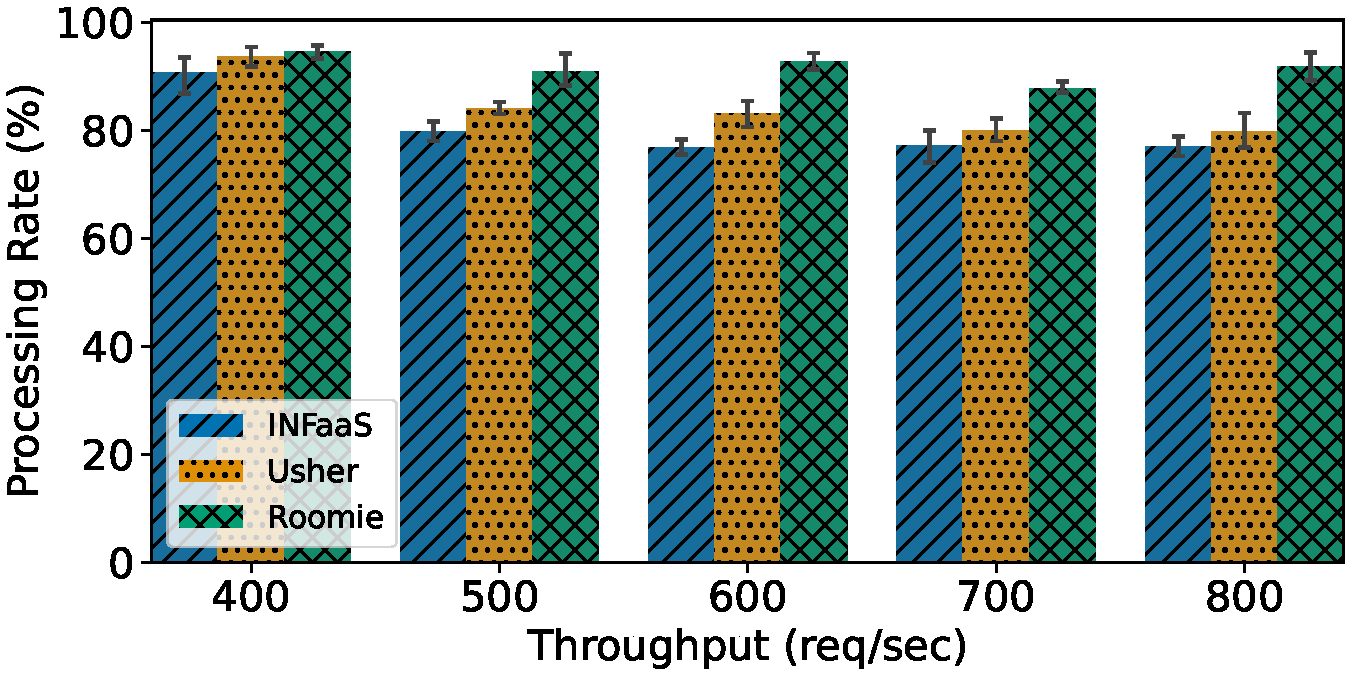
\includegraphics[width=\linewidth]{chapters/roomie/images/JetsonNano/twitter-all-models/normalized.pdf}
		\subcaption{Processing rate.}
	\end{minipage}
	\hfill
	\begin{minipage}[t]{.24\linewidth}
		\centering
		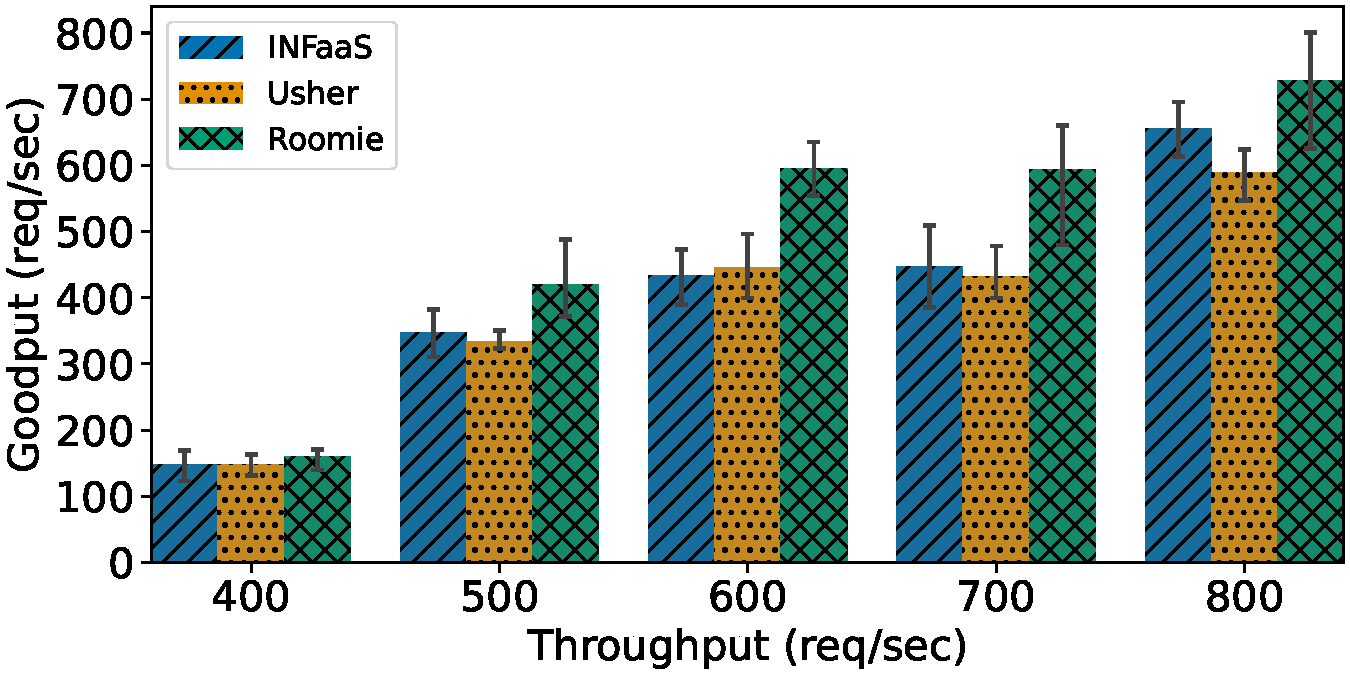
\includegraphics[width=\linewidth]{chapters/roomie/images/JetsonNano/twitter-all-models/goodput.pdf}
		\subcaption{Goodput.}
	\end{minipage}
	\hfill
	\begin{minipage}[t]{.24\linewidth}
		\centering
		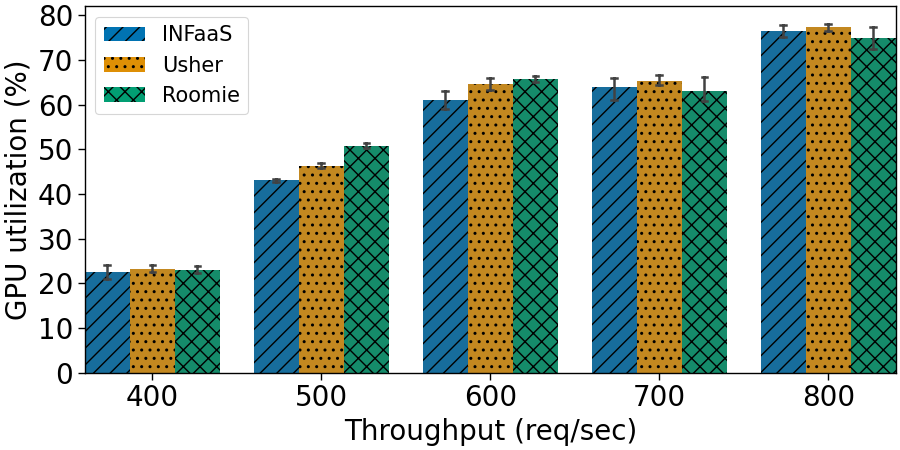
\includegraphics[width=\linewidth]{chapters/roomie/images/JetsonNano/twitter-all-models/gpu_utilization.png}
		\subcaption{GPU utilization.}
	\end{minipage}
	\caption{Edge-based evaluation on the Twitter dataset shows Roomie delivering 8.3× lower latency and superior throughput on Jetson Xavier GPUs, validating its proactive colocation strategy under constrained resources.}
	\label{fig:JetsonNano/twitter-all-models}
	\vspace{-3mm}
\end{figure*}

The~\Cref{fig:JetsonNano/twitter-all-models} presents the results obtained with the Twitter dataset on Jetson Xavier devices. While Usher and INFaaS exhibited similar throughput levels, INFaaS achieved lower latency, whereas Usher maintained a higher processing rate. Roomie, nevertheless, significantly outperformed both, achieving an 8.3× reduction in latency compared to INFaaS under high workload conditions. It also delivered superior throughput and processing rates due to its proactive colocation strategy.

Edge environments impose more severe constraints on model deployment due to limited computing resources and reduced scalability. In this context, Roomie's colocation strategy offers a significant advantage, effectively balancing resource allocation and minimizing performance degradation. As workload intensity increases, GPU utilization increases accordingly, reaching levels significantly higher than those seen in cloud-based configurations. This underscores the critical importance of intelligent colocation policies in edge scenarios, where resource efficiency has a direct impact on system responsiveness and throughput.

\paragraph{Evaluation on synthetic dataset.}

\begin{figure*}
	\begin{minipage}[t]{.24\linewidth}
		\centering
		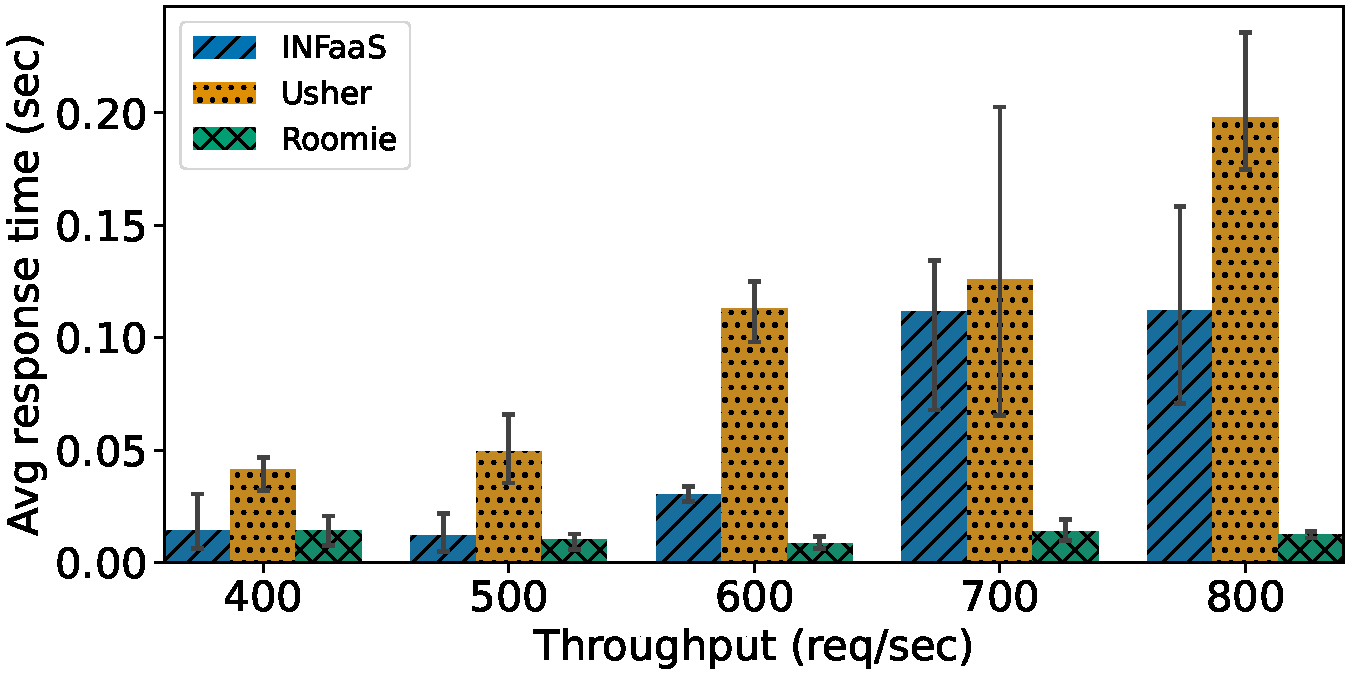
\includegraphics[width=\linewidth]{chapters/roomie/images/JetsonNano/synthetic-all-models/response_time.pdf}
		\subcaption{Response time.}
	\end{minipage}
	\hfill
	\begin{minipage}[t]{.24\linewidth}
		\centering
		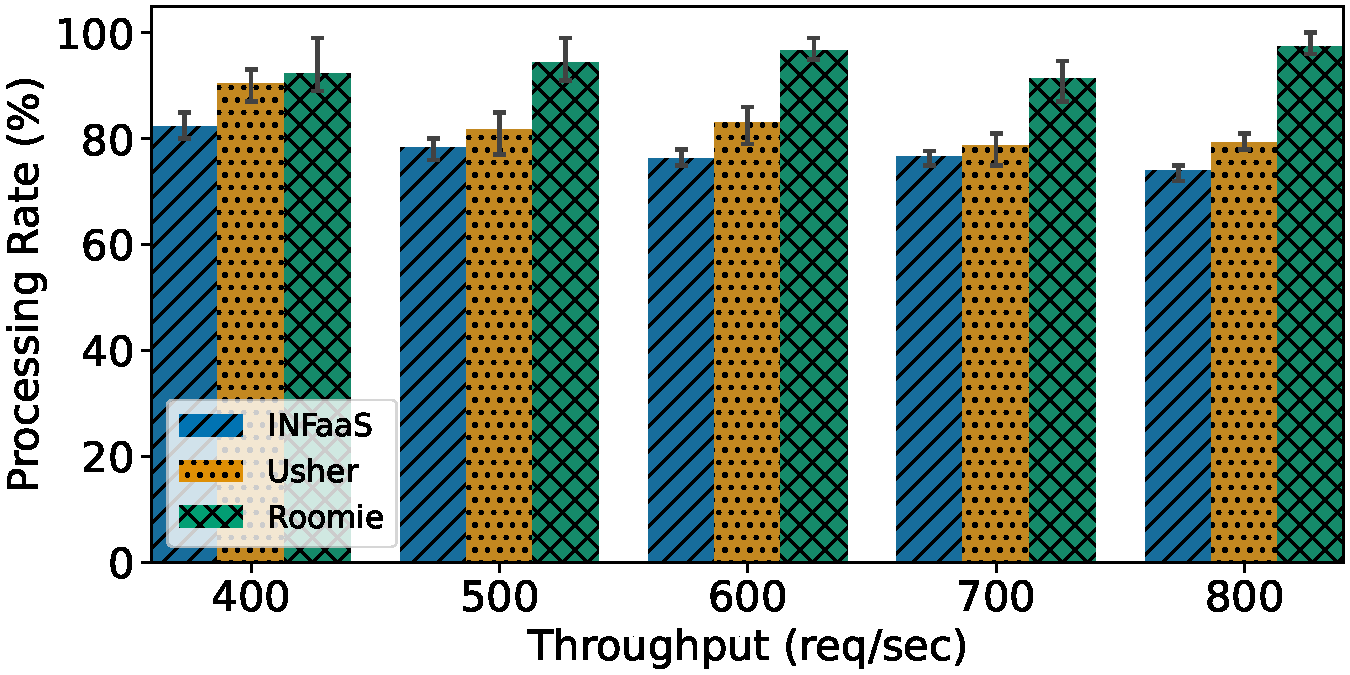
\includegraphics[width=\linewidth]{chapters/roomie/images/JetsonNano/synthetic-all-models/normalized.pdf}
		\subcaption{Processing rate.}
	\end{minipage}
	\hfill
	\begin{minipage}[t]{.24\linewidth}
		\centering
		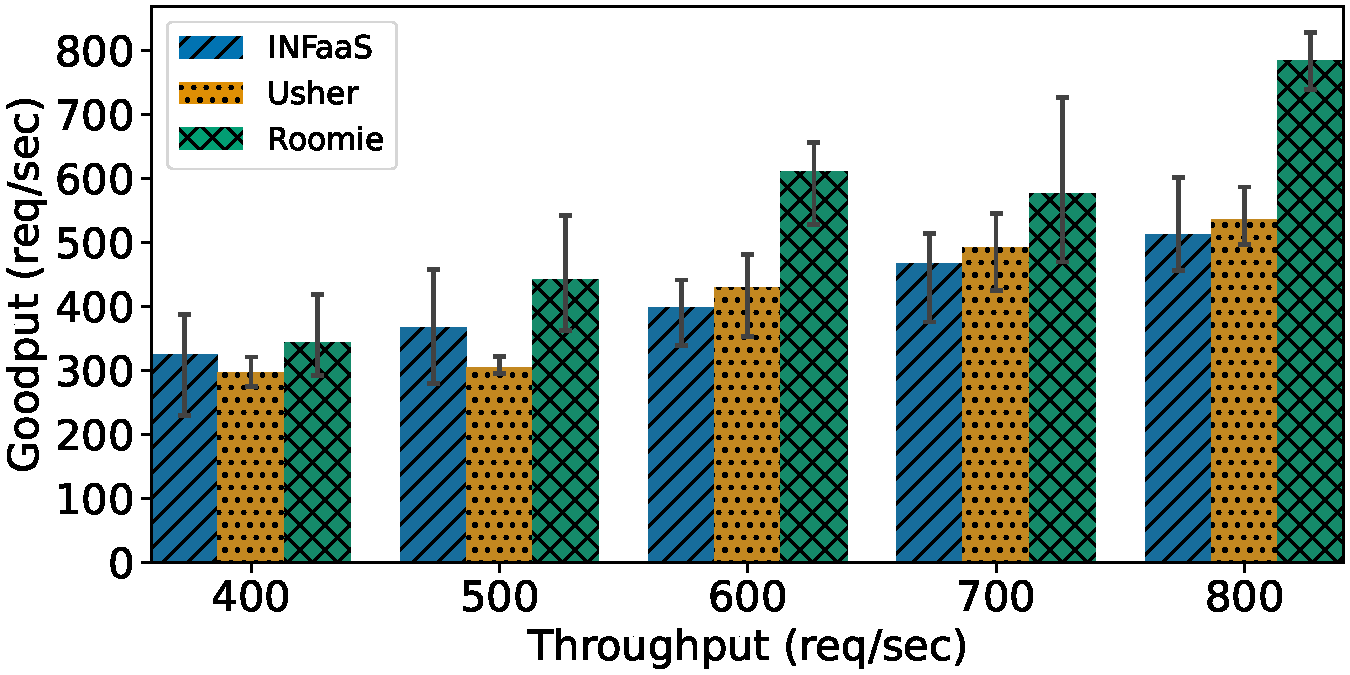
\includegraphics[width=\linewidth]{chapters/roomie/images/JetsonNano/synthetic-all-models/goodput.pdf}
		\subcaption{Goodput.}
	\end{minipage}
	\hfill
	\begin{minipage}[t]{.24\linewidth}
		\centering
		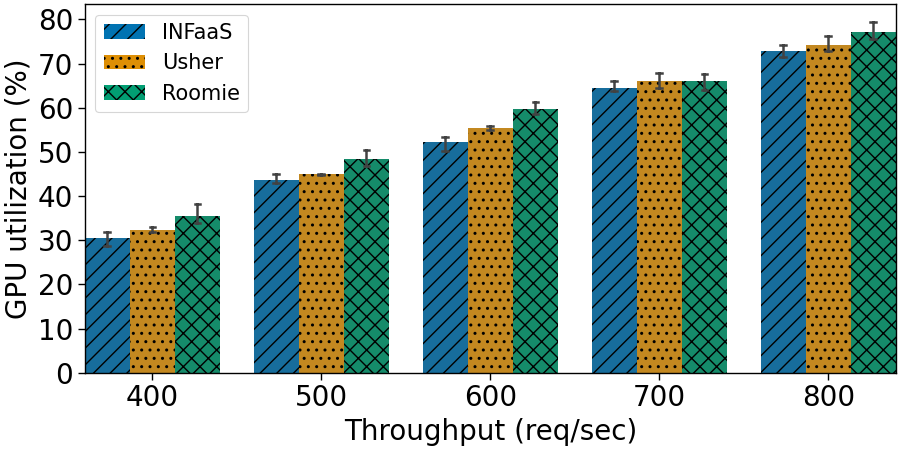
\includegraphics[width=\linewidth]{chapters/roomie/images/JetsonNano/synthetic-all-models/gpu_utilization.png}
		\subcaption{GPU utilization.}
	\end{minipage}
	\caption{Under synthetic edge evaluation, Roomie sustains 9× faster response time and 1.5× higher throughput, demonstrating robust performance in resource-limited environments.}
	\label{fig:JetsonNano/synthetic-all-models}
	\vspace{-3mm}
\end{figure*}

The synthetic dataset evaluation on Jetson Xavier GPUs yielded consistent results with those observed on the Twitter dataset. The results are shown in~\Cref{fig:JetsonNano/synthetic-all-models}. Roomie again demonstrated superior performance, achieving a 9× reduction in response time and a 1.3× increase in processing rate. Throughput was also 1.5× higher than competing approaches.

These findings confirm that Roomie is the most effective DNN deployment strategy in edge computing contexts where colocation is necessary and resources are limited. Its ability to maintain low latency and high throughput under constrained conditions makes it a compelling solution for real-time inference workloads.


\subsection{Roomie: Analyzing Absolute Error in DNN Performance Drop Estimation}

\begin{figure}[t!]
	\centering
	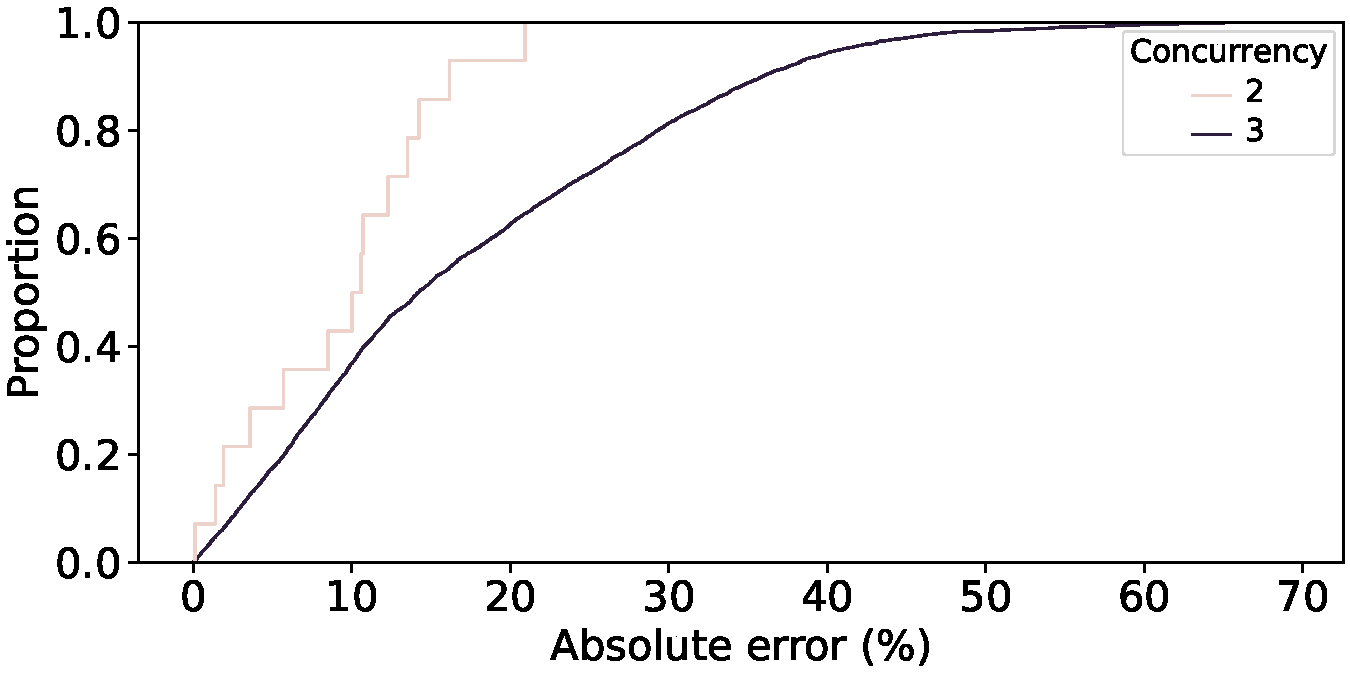
\includegraphics[width=\linewidth]{chapters/roomie/images/absolute_error.pdf}
	\caption{Cumulative distribution of absolute error in estimating performance decline in deep neural networks using Roomie.}
	\label{fig:theoritical_achieved_occupancy}
\end{figure}

The cumulative distribution function (CDF) figure provides insights into the absolute error between the actual performance drop and the estimated performance drop when running 2 or 3 DNNs models on the same GPU.\\
For concurrency of 2, the CDF indicates that a substantial proportion of the absolute errors are below 10.32\%, suggesting that the estimation is relatively accurate for many instances. However, the maximum error of 20.94\% indicates that there are cases where the estimation significantly deviates from the actual performance drop, highlighting potential challenges in accuracy.
In the case of concurrency of 3, the CDF reveals a broader distribution of errors. While there are instances of very low errors, the curve shows that a considerable number of errors exceed 14.24\%, with some reaching as high as 69.14\%.

This variability highlights the increasing difficulty of estimating performance under conditions of high competition, mainly due to the profiling overhead introduced by tools such as Nsight-Compute. Such overhead not only compromises the accuracy of estimates, but also distorts key performance metrics such as kernel execution time, which are central to the modeling process. To promote faster convergence, the heuristic implementation adopts strategies such as pairwise co-location and reduced configuration space. However, these design choices introduce additional complexity when concurrency exceeds two, particularly in modeling how often one model completes inference relative to others. This challenge is further compounded by the presence of interleaved cores and overlapping execution schedules, which obscure clear boundaries in model interactions.

Overall, the analysis indicates that while the estimation method may perform adequately under lower concurrency, the increased complexity and variability at higher concurrency levels can lead to larger discrepancies between estimated and actual performance drops. This underscores the need for careful consideration of profiling overhead when estimating performance in multi-model scenarios on the same GPU.

% \subsection{Ablation Study}
% \label{sec:ablation}

% \paragraph{Kernel-Level Knowledge}

% the performance of the system with and without the kernel-level knowledge

% \paragraph{Model-Level Knowledge}